\documentclass{beamer}

\usetheme{Madrid}

\setbeamertemplate{frame numbering}[fraction]

\usepackage[accumulated]{beamerseminar}
\usepackage[utf8]{inputenc}
\usepackage[english]{babel}
\usepackage{listings}
\usepackage{graphicx,color,pgf}
\usepackage{colortbl}
\usepackage{amsmath,amsfonts,amssymb,amsthm}
\usepackage{latexsym}
\usepackage{outlines}
\usepackage{fourier}
\graphicspath{{./figure/}}

\setbeamertemplate{navigation symbols}{}

\newcommand{\N}{\mathbb{N}}
\newcommand{\Z}{\mathbb{Z}}
\newcommand{\Q}{\mathbb{Q}}
\newcommand{\R}{\mathbb{R}}
\newcommand{\Complessi}{\mathbb{C}}

\theoremstyle{definition}
\newtheorem{defin}{Definition}
\theoremstyle{plain}
\newtheorem{teo}{Theorem}
\newtheorem{prop}{Proposition}
\newtheorem{lemmah}{Lemma}
\newtheorem{cor}{Corollary}
\theoremstyle{Remark}
\newtheorem{oss}{Remark}


\title[]{Graph-based approaches for Demonstration selection in In-Context
	Learning}
	\subtitle{Comparative experiments with the Chef's Hat card game}
\author[]{Francesco Alfieri \\ francesco.alfieri5@studio.unibo.it}

\date{28/01/2025}

\definecolor{light-gray}{gray}{0.95} 

\begin{document}
	
	\begin{frame}
		\titlepage
	\end{frame}
	
	\begin{frame}
		\frametitle{Introduction}
		
		We perform experiments about the capabilities of LLMs to understand the legality of moves in board games via In-Context Learning, specifically focusing on Demonstration Selection.
		
		\bigskip
		
		The specific board game we focus on  is \emph{Chef's Hat} (https://whisperproject.eu/chefshat):
		
		\bigskip
		\pause
		Two main advantages:\pause
		\begin{itemize}
			\item Simple game;\pause
			\item Lack of literature with respect to more famous games (e.g. Chess, Othello).
		\end{itemize}
		
	\end{frame}
	
	%%%%%%%%%%%%%%%%%%%%%%%%%%%%%%%%%%%%%%%%%%%%%%%%%%%%%%%%%%%%%%%%%%%%%%%%%%%%%%%%%%%%%%%%%%%%%
	
	\begin{frame}
		
		\frametitle{Chef's Hat}
		\pause
		There are three phases per round (\emph{Shift}):
		\pause
		\begin{enumerate}
			\item Start of the Shift: cards and roles are dealt to the players. Players exchange up to 2 cards with each other depending on their role;\pause 
			\item Making Pizzas: The bulk of the game. Players take turns in placing cards according to the rules on the board until all of them empty their hands;\pause
			\item End of Shift: a cleanup step where points are scored and roles are reassigned. No players' agency in this phase.\pause
		\end{enumerate}\bigskip
		
		We deal with the second phase only.
		
	\end{frame}
	
	%%%%%%%%%%%%%%%%%%%%%%%%%%%%%%%%%%%%%%%%%%%%%%%%%%%%%%%%%%%%%%%%%%%%%%%%%%%%%%%%%%%%%%%%%%%%%
	
	%\begin{frame}
	%	\frametitle{Making Pizzas}
	%	\pause
	%	Rules for playing cards: \pause
	%	\begin{enumerate}
	%		\item  The played cards need to have lower face values
	%		than the previously played cards and they have to be placed above the cards on the board;\pause
	%		\item Players can play
	%		multiple copies of a card at once;\pause
	%		\item Players always have
	%		to play an equal or greater amount of copies than
	%		the previous player did; \pause
	%		\item Players always have the chance to \emph{pass} their turn until the next \emph{pizza}, whether or not they can play cards.
			
	%\end{enumerate}
	%\end{frame}
	
	%%%%%%%%%%%%%%%%%%%%%%%%%%%%%%%%%%%%%%%%%%%%%%%%%%%%%%%%%%%%%%%%%%%%%%%%%%%%%%%%%%%%%%%%%%%%%
	
	\begin{frame}
		\frametitle{The Data}
		A total of 7819 unique triples of the form (\emph{Player\_Hand}, \emph{Board\_Before}, \emph{Possible\_Actions}) obtained by letting four agents which choose random moves play against each other for 100 matches.\pause \bigskip
		
		We only use the 221 triples from the last 3 matches as a test set.\pause \bigskip
		
		The first two are lists of 17 and 11 natural numbers from 0 to 13. All elements represent the value of a card, except for 0 (missing card) and 12 (Joker card).\pause \bigskip
		
		Possible\_Actions are lists of elements CX;QY;JZ and \emph{pass}, where the former represents the move
		which consists in playing Y cards with value X and
		Z Joker cards. \pause\bigskip
		
		We feed prompts that are made of 3 different templates of increasing complexity with 5/10/15 pairs of game states and corresponding legal moves to Llama 3.1 8B Instruct.
		
	\end{frame}
	
	%%%%%%%%%%%%%%%%%%%%%%%%%%%%%%%%%%%%%%%%%%%%%%%%%%%%%%%%%%%%%%%%%%%%%%%%%%%%%%%%%%%%%%%%%%%%%
	\begin{frame}
		\frametitle{Example}
		
		Player Hand: (0, 0, 5, 6, 7, 7, 7, 8, 9, 9, 9, 10, 10, 10,
		11, 11, 11);\bigskip
		
		
		Board State: (13, 0, 0, 0, 0, 0, 0, 0, 0, 0, 0)\bigskip
		
		
		Legal moves:  [’C5;Q1;J0’, ’C6;Q1;J0’, ’C7;Q1;J0’,
		’C7;Q2;J0’, ’C7;Q3;J0’, ’C8;Q1;J0’,
		’C9;Q1;J0’, ’C9;Q2;J0’, ’C9;Q3;J0’,
		’C10;Q1;J0’, ’C10;Q2;J0’, ’C10;Q3;J0’,
		’C11;Q1;J0’, ’C11;Q2;J0’, ’C11;Q3;J0’,
		’pass’]
		
		
	\end{frame}
	
	
	%%%%%%%%%%%%%%%%%%%%%%%%%%%%%%%%%%%%%%%%%%%%%%%%%%%%%%%%%%%%%%%%%%%%%%%%%%%%%%%%%%%%%%%%%%%%%
	\begin{frame}
		\frametitle{Objectives}
		
		\pause
		It has been observed that choosing close examples that are semantically relevant
		to test instances via KNN (in the embedding space, either via euclidean distance or cosine similarity) can greatly improve the performance of ICL.\pause \bigskip
		
		On the other hand, semantic diversity between demonstrations has also been shown to play a key role in ICL performances.
		
		We propose graph-based approaches to demonstration selection with the goal of choosing examples that are:\pause
		\begin{enumerate}
			\item Relevant to a given query;\pause
			\item Good summaries of abstract concepts of all the available examples;\pause
			\item Diverse to each other.
		\end{enumerate}
		
		
	\end{frame}
	%%%%%%%%%%%%%%%%%%%%%%%%%%%%%%%%%%%%%%%%%%%%%%%%%%%%%%%%%%%%%%%%%%%%%%%%%%%%%%%%%%%%%%%%%%%%%
	\begin{frame}
		\frametitle{Graph Theory Tools}
	\pause
	\begin{columns}
		\begin{column}{0.5\textwidth}
	We mainly use two tools from graph theory:\pause
	\begin{enumerate}
		\item The PageRank centrality measure: a variant of eigenvector centrality;\pause
		\item The Louvain method for community detection: a fast heuristic method for partitioning graphs in communities with high modularity.\pause
	\end{enumerate}\end{column}
		\begin{column}{0.5\textwidth}
	\begin{figure}
		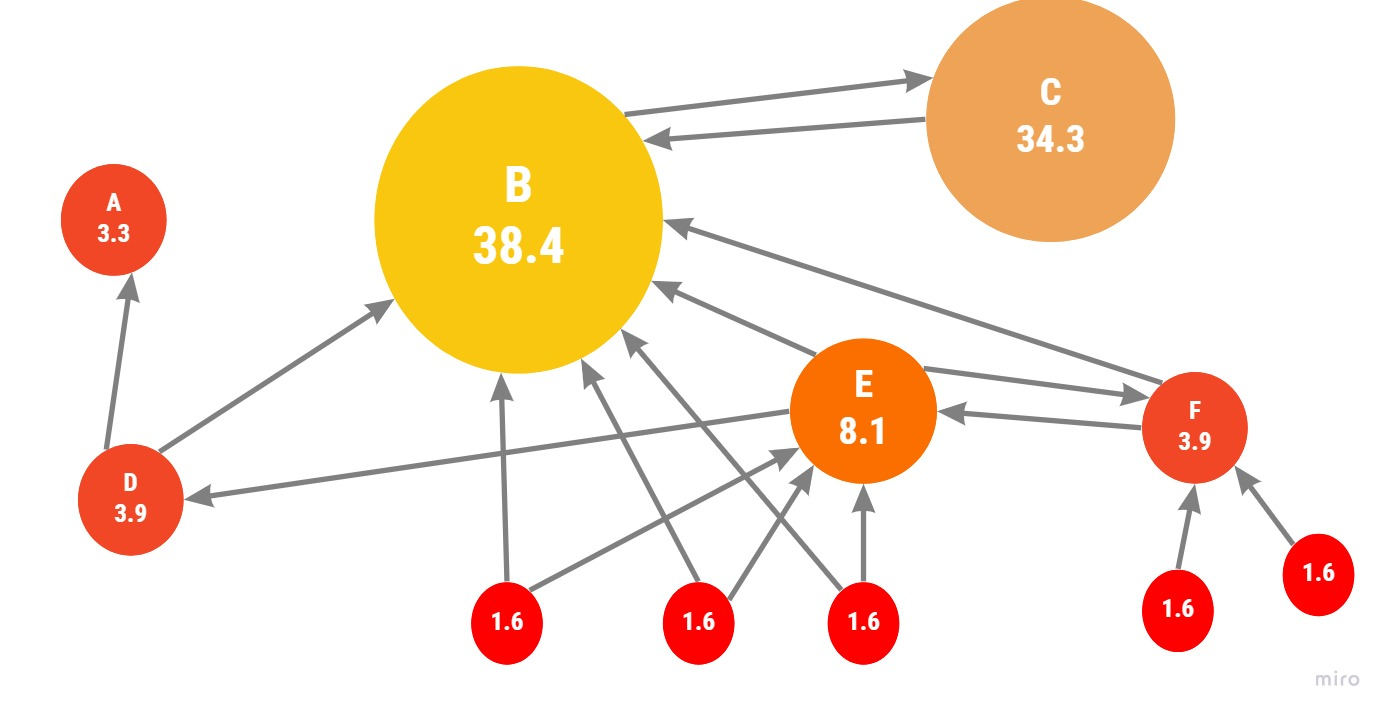
\includegraphics[height=3cm, width=5cm]{pagerank.jpg}
	\end{figure}
	\begin{figure}
		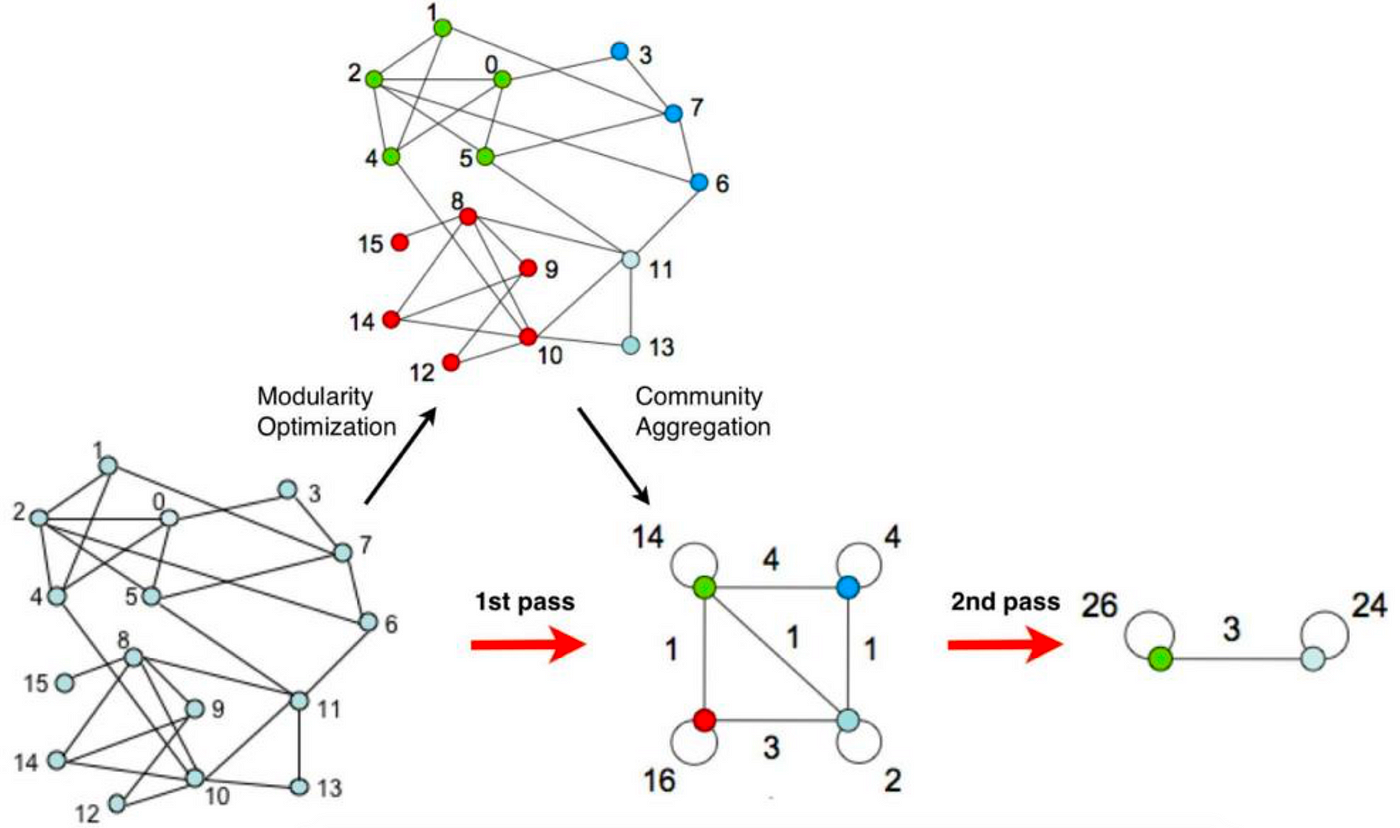
\includegraphics[height=3cm, width=5cm]{louvain.png}

	\end{figure}

\end{column}
	\end{columns}
		
		
	\end{frame}
	%%%%%%%%%%%%%%%%%%%%%%%%%%%%%%%%%%%%%%%%%%%%%%%%%%%%%%%%%%%%%%%%%%%%%%%%%%%%%%%%%%%%%%%%%%%%%	
	%%%%%%%%%%%%%%%%%%%%%%%%%%%%%%%%%%%%%%%%%%%%%%%%%%%%%%%%%%%%%%%%%%%%%%%%%%%%%%%%%%%%%%%%%%%%%
	\begin{frame}
		\frametitle{Main approach}
		The proposed approach follows these steps:
		\begin{enumerate}
			\item Build the \emph{Demonstration Graph} according to a \emph{resolution} parameter $R$;\pause
			\item For each test instance, extract a subgraph of the \emph{Demonstration Graph} according to a \emph{radius} parameter $r$;\pause
			\item Return the top 5/10/15 demonstrations from the extracted subgraph according to the PageRank metric.\pause
		\end{enumerate}
		
		\begin{block}{Observation}
			If links between nodes represent similarity, the nodes with the highest PageRank scores are the most similar to nodes that are similar to many nodes.
			\end{block}\pause
		
	We use the Hamming distance between concatenations of Board states and Players' hands.
		
	\end{frame}
	%%%%%%%%%%%%%%%%%%%%%%%%%%%%%%%%%%%%%%%%%%%%%%%%%%%%%%%%%%%%%%%%%%%%%%%%%%%%%%%%%%%%%%%%%%%%%
	
	\begin{frame}
		\frametitle{Variants}
		\pause
		\begin{enumerate}
			\item Add weights to edges $(i,j)$ monotonically decreasing with respect to $d(i,j)$;\pause
			\item Use the Louvain method on the extracted subgraph and return the top nodes (PageRank-wise) from the largest detected communities.\pause \bigskip
		\end{enumerate}
	\begin{block}{Observation}
		The Louvain variant aims at increasing the diversity between prompted demonstrations.
	\end{block}
	\end{frame}
	%%%%%%%%%%%%%%%%%%%%%%%%%%%%%%%%%%%%%%%%%%%%%%%%%%%%%%%%%%%%%%%%%%%%%%%%%%%%%%%%%%%%%%%%%%%%%
	
	\begin{frame}
		\frametitle{Results}
		\begin{table}[H]
			\resizebox{\columnwidth}{!}{%
				\begin{tabular}{|l|l|lll|lll|lll|}
					\cline{1-1} \cline{3-11}
					\multicolumn{1}{|c|}{\textit{}} &
					&
					\multicolumn{3}{c|}{\textit{Minimal template}} &
					\multicolumn{3}{l|}{\textit{Intermediate template}} &
					\multicolumn{3}{l|}{\textit{Complex Template}} \\ \cline{1-1} \cline{3-11} 
					\# of examples &
					&
					\multicolumn{1}{l|}{5} &
					\multicolumn{1}{l|}{10} &
					15 &
					\multicolumn{1}{l|}{5} &
					\multicolumn{1}{l|}{10} &
					15 &
					\multicolumn{1}{l|}{5} &
					\multicolumn{1}{l|}{10} &
					15 \\ \cline{1-1} \cline{3-11} 
					&
					&
					\multicolumn{1}{l|}{} &
					\multicolumn{1}{l|}{} &
					&
					\multicolumn{1}{l|}{} &
					\multicolumn{1}{l|}{} &
					&
					\multicolumn{1}{l|}{} &
					\multicolumn{1}{l|}{} &
					\\ \cline{1-1} \cline{3-11} 
					Random baseline &
					&
					\multicolumn{1}{l|}{.259} &
					\multicolumn{1}{l|}{.205} &
					.265 &
					\multicolumn{1}{l|}{.259} &
					\multicolumn{1}{l|}{.277} &
					.312 &
					\multicolumn{1}{l|}{.163} &
					\multicolumn{1}{l|}{.201} &
					.240 \\ \cline{1-1} \cline{3-11} 
					KNN baseline &
					&
					\multicolumn{1}{l|}{.431} &
					\multicolumn{1}{l|}{.441} &
					.462 &
					\multicolumn{1}{l|}{.434} &
					\multicolumn{1}{l|}{.470} &
					.486 &
					\multicolumn{1}{l|}{.270} &
					\multicolumn{1}{l|}{.374} &
					.408 \\ \cline{1-1} \cline{3-11} 
				\end{tabular}%
			}
			\caption{IoU scores of the two baselines.}
			\label{iou base}
		\end{table}
	\end{frame}
	\begin{frame}
				\frametitle{Results}
		\begin{table}
			\resizebox{\columnwidth}{!}{%
				\begin{tabular}{|l|l|lll|lll|lll|}
					\cline{1-1} \cline{3-11}
					\multicolumn{1}{|c|}{\textit{}} &
					&
					\multicolumn{3}{c|}{\textit{Minimal template}} &
					\multicolumn{3}{l|}{\textit{Intermediate template}} &
					\multicolumn{3}{l|}{\textit{Complex Template}} \\ \cline{1-1} \cline{3-11} 
					\# of examples &
					&
					\multicolumn{1}{l|}{5} &
					\multicolumn{1}{l|}{10} &
					15 &
					\multicolumn{1}{l|}{5} &
					\multicolumn{1}{l|}{10} &
					15 &
					\multicolumn{1}{l|}{5} &
					\multicolumn{1}{l|}{10} &
					15 \\ \cline{1-1} \cline{3-11} 
					&
					&
					\multicolumn{1}{l|}{} &
					\multicolumn{1}{l|}{} &
					&
					\multicolumn{1}{l|}{} &
					\multicolumn{1}{l|}{} &
					&
					\multicolumn{1}{l|}{} &
					\multicolumn{1}{l|}{} &
					\\ \cline{1-1} \cline{3-11} 
					R=5; r=10 &
					&
					\multicolumn{1}{l|}{.271} &
					\multicolumn{1}{l|}{.300} &
					.329 &
					\multicolumn{1}{l|}{.284} &
					\multicolumn{1}{l|}{.309} &
					.309 &
					\multicolumn{1}{l|}{.208} &
					\multicolumn{1}{l|}{.259} &
					.278 \\ \cline{1-1} \cline{3-11} 
					R=5; r=6 &
					&
					\multicolumn{1}{l|}{.376} &
					\multicolumn{1}{l|}{.392} &
					.395 &
					\multicolumn{1}{l|}{.366} &
					\multicolumn{1}{l|}{\textbf{.405}} &
					.394 &
					\multicolumn{1}{l|}{.275} &
					\multicolumn{1}{l|}{.321} &
					.338 \\ \cline{1-1} \cline{3-11} 
					R=4; r=8 &
					&
					\multicolumn{1}{l|}{.326} &
					\multicolumn{1}{l|}{.324} &
					.357 &
					\multicolumn{1}{l|}{.300} &
					\multicolumn{1}{l|}{.328} &
					.350 &
					\multicolumn{1}{l|}{.226} &
					\multicolumn{1}{l|}{.306} &
					.313 \\ \cline{1-1} \cline{3-11} 
					R=4; r=6 &
					&
					\multicolumn{1}{l|}{.365} &
					\multicolumn{1}{l|}{.378} &
					.368 &
					\multicolumn{1}{l|}{.352} &
					\multicolumn{1}{l|}{.387} &
					.382 &
					\multicolumn{1}{l|}{\textbf{.299}} &
					\multicolumn{1}{l|}{\textbf{.338}} &
					.355 \\ \cline{1-1} \cline{3-11} 
					R=3; r=8 &
					&
					\multicolumn{1}{l|}{.308} &
					\multicolumn{1}{l|}{.322} &
					.354 &
					\multicolumn{1}{l|}{.315} &
					\multicolumn{1}{l|}{.342} &
					.351 &
					\multicolumn{1}{l|}{.220} &
					\multicolumn{1}{l|}{.287} &
					.315 \\ \cline{1-1} \cline{3-11} 
					R=3; r=6 &
					&
					\multicolumn{1}{l|}{.347} &
					\multicolumn{1}{l|}{.362} &
					.390 &
					\multicolumn{1}{l|}{.330} &
					\multicolumn{1}{l|}{.366} &
					.396 &
					\multicolumn{1}{l|}{.272} &
					\multicolumn{1}{l|}{.315} &
					.340 \\ \cline{1-1} \cline{3-11} 
					Louvain; R=5; r=6 &
					&
					\multicolumn{1}{l|}{\textbf{.379}} &
					\multicolumn{1}{l|}{\textbf{.398}} &
					\textbf{.401} &
					\multicolumn{1}{l|}{\textbf{.384}} &
					\multicolumn{1}{l|}{.400} &
					\textbf{.416} &
					\multicolumn{1}{l|}{.256} &
					\multicolumn{1}{l|}{.333} &
					\textbf{.376} \\ \cline{1-1} \cline{3-11} 
					weighted; R=5, r=6 &
					&
					\multicolumn{1}{l|}{.370} &
					\multicolumn{1}{l|}{.384} &
					.385 &
					\multicolumn{1}{l|}{.347} &
					\multicolumn{1}{l|}{.385} &
					.376 &
					\multicolumn{1}{l|}{.265} &
					\multicolumn{1}{l|}{.331} &
					.353 \\ \cline{1-1} \cline{3-11}
				\end{tabular}%
			}
			\caption{IoU scores for fixed-radius approaches with various parameter configurations. Results suggests that subgraphs with a smaller radius $r$ behave generally better. On the other hand, denser demonstration graphs with higher resolution $R$ achieve better performance. The Louvain method outperforms all other approaches in most cases.}
			\label{iou fixed}
			\end{table}
	\end{frame}
	
	%%%%%%%%%%%%%%%%%%%%%%%%%%%%%%%%%%%%%%%%%%%%%%%%%%%%%%%%%%%%%%%%%%%%%%%%%%%%%%%%%%%%%%%%%%%%%

	\begin{frame}
		\frametitle{Results}
	\begin{table}[H]
		\resizebox{\columnwidth}{!}{%
			\begin{tabular}{|l|l|lll|lll|lll|}
				\hline
				\multicolumn{1}{|c|}{\textit{}} &
				&
				\multicolumn{3}{c|}{\textit{Minimal template}} &
				\multicolumn{3}{l|}{\textit{Intermediate template}} &
				\multicolumn{3}{l|}{\textit{Complex Template}} \\ \hline
				\# of examples &
				&
				\multicolumn{1}{l|}{5} &
				\multicolumn{1}{l|}{10} &
				15 &
				\multicolumn{1}{l|}{5} &
				\multicolumn{1}{l|}{10} &
				15 &
				\multicolumn{1}{l|}{5} &
				\multicolumn{1}{l|}{10} &
				15 \\ \hline
				&
				&
				\multicolumn{1}{l|}{} &
				\multicolumn{1}{l|}{} &
				&
				\multicolumn{1}{l|}{} &
				\multicolumn{1}{l|}{} &
				&
				\multicolumn{1}{l|}{} &
				\multicolumn{1}{l|}{} &
				\\ \hline
				R=3 &
				&
				\multicolumn{1}{l|}{\textbf{.417}} &
				\multicolumn{1}{l|}{.425} &
				\textbf{.446} &
				\multicolumn{1}{l|}{\textbf{.431}} &
				\multicolumn{1}{l|}{\textbf{.447}} &
				\textbf{.466} &
				\multicolumn{1}{l|}{.259} &
				\multicolumn{1}{l|}{.351} &
				.391 \\ \hline
				R=5 &
				&
				\multicolumn{1}{l|}{.404} &
				\multicolumn{1}{l|}{.402} &
				.425 &
				\multicolumn{1}{l|}{.421} &
				\multicolumn{1}{l|}{\textbf{.447}} &
				.456 &
				\multicolumn{1}{l|}{\textbf{.284}} &
				\multicolumn{1}{l|}{.350} &
				.380 \\ \hline
				weighted; R=3 &
				&
				\multicolumn{1}{l|}{.406} &
				\multicolumn{1}{l|}{.419} &
				.437 &
				\multicolumn{1}{l|}{.405} &
				\multicolumn{1}{l|}{.421} &
				.455 &
				\multicolumn{1}{l|}{.244} &
				\multicolumn{1}{l|}{.345} &
				\textbf{.394} \\ \hline
				weighted; R=5 &
				&
				\multicolumn{1}{l|}{.392} &
				\multicolumn{1}{l|}{.416} &
				.435 &
				\multicolumn{1}{l|}{.376} &
				\multicolumn{1}{l|}{.404} &
				.449 &
				\multicolumn{1}{l|}{.230} &
				\multicolumn{1}{l|}{.337} &
				.363 \\ \hline
				Louvain; R=3 &
				&
				\multicolumn{1}{l|}{.415} &
				\multicolumn{1}{l|}{\textbf{.444}} &
				.423 &
				\multicolumn{1}{l|}{.422} &
				\multicolumn{1}{l|}{.419} &
				.434 &
				\multicolumn{1}{l|}{.261} &
				\multicolumn{1}{l|}{.332} &
				.373 \\ \hline
				Louvain; R=5 &
				&
				\multicolumn{1}{l|}{.399} &
				\multicolumn{1}{l|}{.404} &
				.409 &
				\multicolumn{1}{l|}{.424} &
				\multicolumn{1}{l|}{.442} &
				.452 &
				\multicolumn{1}{l|}{.249} &
				\multicolumn{1}{l|}{\textbf{.354}} &
				.380 \\ \hline
			\end{tabular}%
		}
		\caption{IoU scores for smallest-radius subgraph approaches with different values for Resolution $R$. Contrary to the observations from Table \ref{iou fixed}, it seems that for very small subgraphs, sparser demonstration graphs prove more effective.}
		\label{iou iterative}
	\end{table}
	
	\end{frame}
	%%%%%%%%%%%%%%%%%%%%%%%%%%%%%%%%%%%%%%%%%%%%%%%%%%%%%%%%%%%%%%%%%%%%%%%%%%%%%%%%%%%%%%%%%%%%%
	
	\begin{frame}
		\frametitle{A candidate explanation}
		The results show that in this case closeness to the test instances is the most impactful factor in performances, while other parameters and approaches produce marginal differences.\pause \bigskip
		
		This is probably due to a poor choice of distance: game states with a Hamming distance of 1 can have vastly different sequences of legal moves. \pause \bigskip
		
		This effect quickly becomes larger and larger as the Hamming distance increases.
		

		
		
		
		
		
	\end{frame}
		%%%%%%%%%%%%%%%%%%%%%%%%%%%%%%%%%%%%%%%%%%%%%%%%%%%%%%%%%%%%%%%%%%%%%%%%%%%%%%%%%%%%%%%%%%%%%
		
	\begin{frame}
		\frametitle{Further developments}
		A number of topics can be further investigated:\pause
		\begin{itemize}
			\item Different choice of metric;\pause
			\item Different choice of node scoring;\pause
			\item Systematic ways to set parameters $R$ and $r$;\pause
			\item For weighted approaches, a different degradation method of the weights;\pause
			\item For the Louvain method, a systematic way to choose the resolution parameter $\gamma$;\pause
			\item Alternatives to the Louvain method for (potentially overlapping) community detection;\pause
			\item Use of different LLMs.\pause
			\item Application of the methods to different, more popular, domains.
		\end{itemize}
		
	\end{frame}
	%%%%%%%%%%%%%%%%%%%%%%%%%%%%%%%%%%%%%%%%%%%%%%%%%%%%%%%%%%%%%%%%%%%%%%%%%%%%%%%%%%%%%%%%%%%%%
\begin{frame}
	\begin{center}
			Thank you for your attention!
	\end{center}

\end{frame}

	
\end{document}
